% для компиляции в lualatex!!
%\documentclass[12pt, a4paper]{article}
\documentclass[12pt, a4paper]{disser}
\usepackage[english,russian]{babel}
\usepackage[warn]{mathtext}
%\usepackage[T2A]{fontenc}
%\usepackage[utf8]{inputenc}

\usepackage{xecyr} % Продукт Вашего покорного слуги ;)

%\setmainfont{DejaVu Serif}
\setmainfont{Liberation Serif}

\usepackage{color}
\usepackage{amssymb,amsmath}
\usepackage{graphicx}
\usepackage{multicol}

\textheight=24cm           % высота текста
\textwidth=16cm            % ширина текста
\oddsidemargin=0pt         % отступ от левого края
\topmargin=-1.5cm          % отступ от верхнего края
\parindent=24pt            % абзацный отступ
\parskip=0pt               % интервал между абзацами
\tolerance=2000            % терпимость к "жидким" строкам
\flushbottom               % выравнивание высоты страниц
%\def\baselinestretch{1.5} % печать с большим интервалом

%\title{}
%\author{\copyright~~С.А.~Назарова \thanks{e-mail:~sophia.nazarova@gmail.com}}
%\date{}


\begin{document}

	\section{Динамика обилия {\it M.~balthica}.}

		\subsection{Эстуарий реки~Лувеньги.}


На литорали в эстуарии р.~Лувеньги средняя плотность поселений маком за период с $1992$ по $2012$ год колебалась от $55~(26,8)$ в $1992$ до $9200~(39,8)$~экз./м$^2$ в $1998$ году (рис. \ref{ris:dynamic_Kandalaksha_all}). 
	\begin{figure}[h]
	
	\begin{minipage}[b]{.46\linewidth}
	%Фигурка в первом ряду слева размер отведенный под весь этот объект \textendash 0.46 от ширины строки
	%Параметр [b] означает, что выравнивание этих министраниц будет по нижнему краю
	\begin{center}
		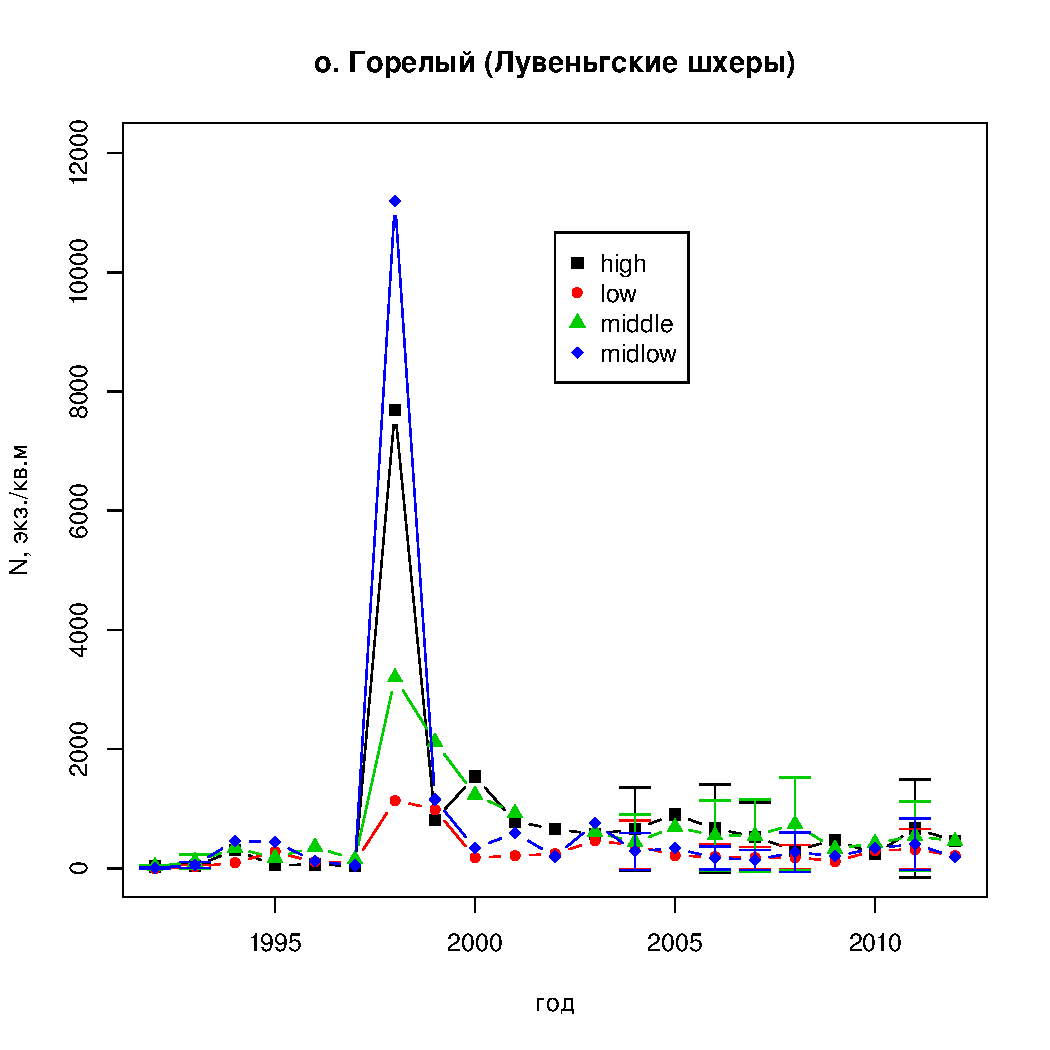
\includegraphics[width=65mm]{../White_Sea/Luvenga_Goreliy/N_dynamic.pdf}
	\end{center}
	\end{minipage}
	%
	\hfil %Это пружинка отодвигающая рисунки друг от друга
	%
	\begin{minipage}[b]{.46\linewidth}
%Следующий рисунок - первый ряд справа %DUNGEON S_4 \ AB
	\begin{center}
		\includegraphics[width=65mm]{../White_Sea//Luvenga_II_razrez/N_dynamic.pdf}
	\end{center}
	\end{minipage}

%\smallskip


	\begin{minipage}[b]{.46\linewidth}
%Фигурка в первом ряду слева размер отведенный под весь этот объект \textendash 0.46 от ширины строки
%Параметр [b] означает, что выравнивание этих министраниц будет по нижнему краю
	\begin{center}
	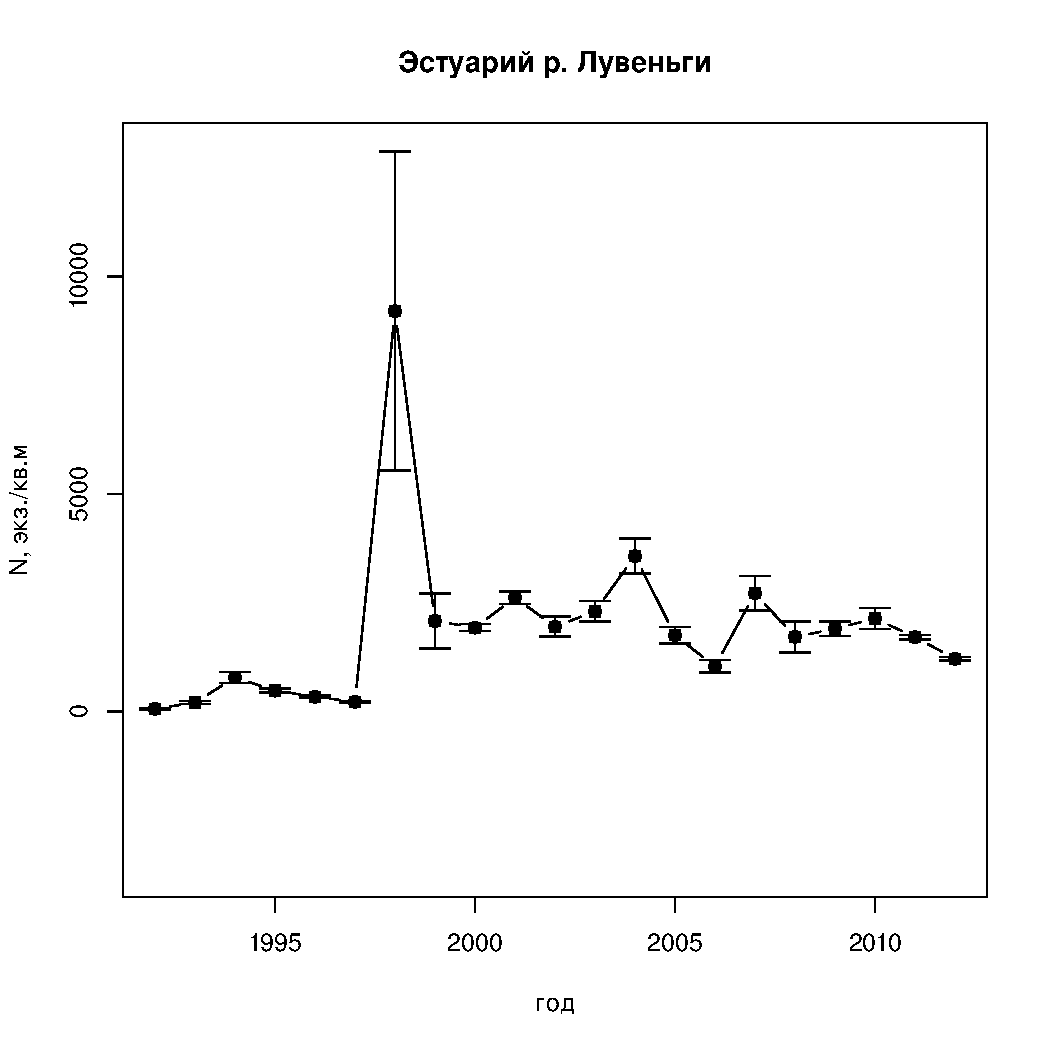
\includegraphics[width=65mm]{../White_Sea/Estuatiy_Luvenga/N_dynamic.pdf}
	\end{center}
	\end{minipage}
%
	\hfil %Это пружинка отодвигающая рисунки друг от друга
%
	\begin{minipage}[b]{.46\linewidth}
%Следующий рисунок - первый ряд справа %DUNGEON S_4 \ AB
	\begin{center}
		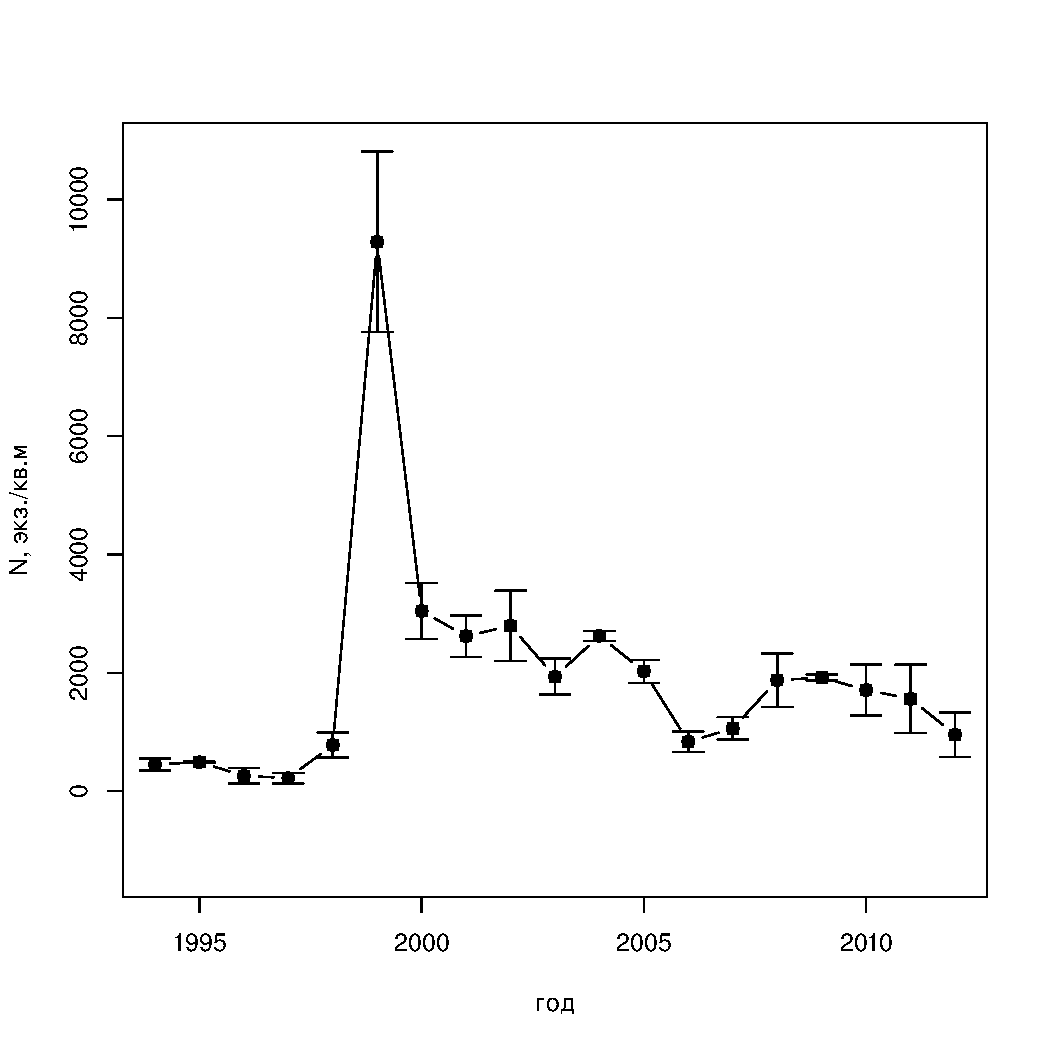
\includegraphics[width=65mm]{../White_Sea/Ryashkov_ZRS/N_dynamic.pdf}
	\end{center}
	\end{minipage}

%\smallskip

	\begin{minipage}[b]{.46\linewidth}
%Фигурка в первом ряду слева размер отведенный под весь этот объект \textendash 0.46 от ширины строки
%Параметр [b] означает, что выравнивание этих министраниц будет по нижнему краю
	\begin{center}
		\includegraphics[width=65mm]{../White_Sea/Ryashkov_YuG/N_dynamic.pdf}
	\end{center}
	\end{minipage}
%
	\hfil %Это пружинка отодвигающая рисунки друг от друга
%
	\begin{minipage}[b]{.46\linewidth}
%Следующий рисунок - первый ряд справа %DUNGEON S_4 \ AB
	\begin{center}
		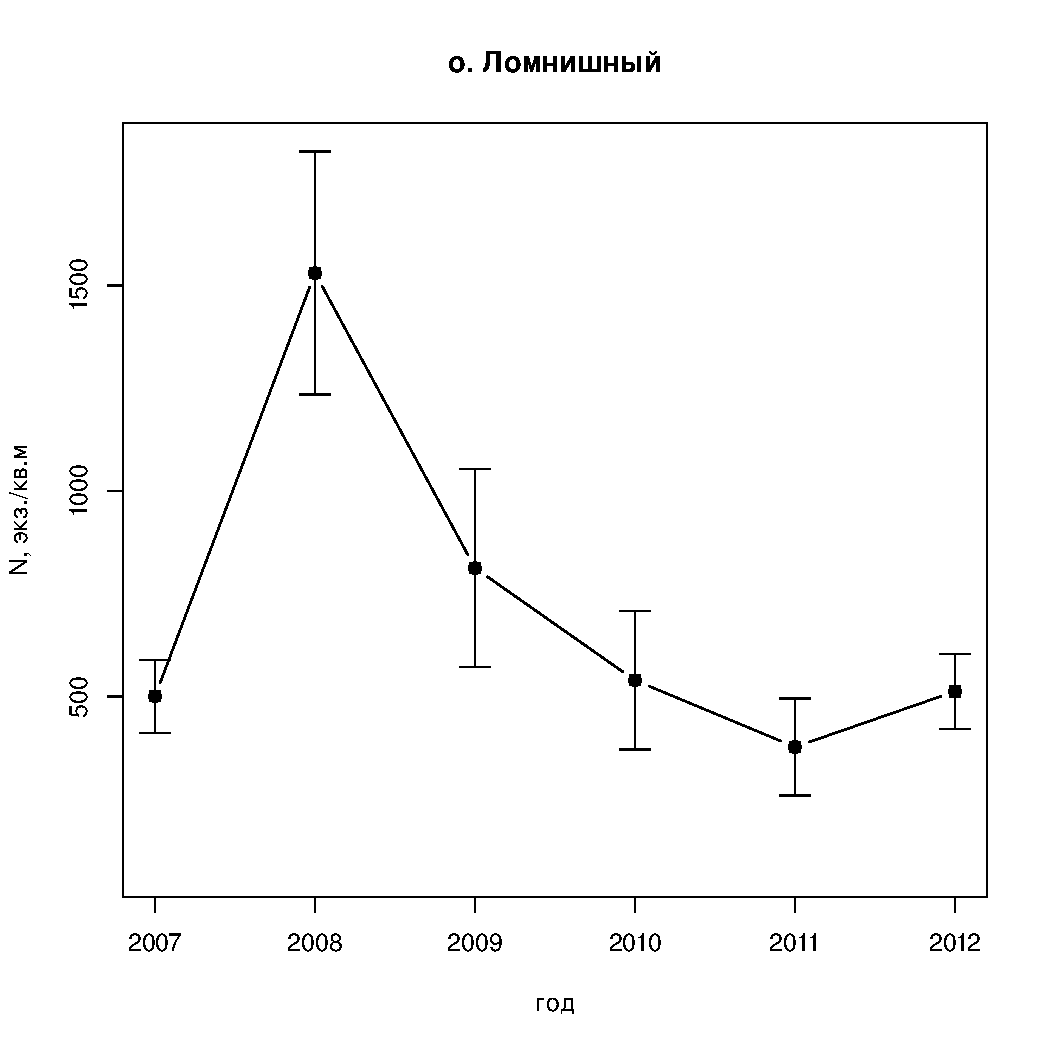
\includegraphics[width=65mm]{../White_Sea/Lomnishniy/N_dynamic.pdf}
	\end{center}
	\end{minipage}

%\smallskip


	\caption{Динамика плотности поселений {\it Macoma balthica} в вершине Кандалакшского залива}
	\label{ris:dynamic_Kandalaksha_all}
	\end{figure}
При этом столь высокая численность в $1998$ году была связана с особями длиной менее $1$~мм (рис. \ref{ris:dynamic_Kandalaksha_all2}) \textemdash средняя численность моллюсков крупнее $1$~мм составляла всего $750~(2,03)$~экз./м$^2$.
	\begin{figure}[h]

	\begin{minipage}[b]{.46\linewidth}
%Фигурка в первом ряду слева размер отведенный под весь этот объект \textendash 0.46 от ширины строки
%Параметр [b] означает, что выравнивание этих министраниц будет по нижнему краю
	\begin{center}
		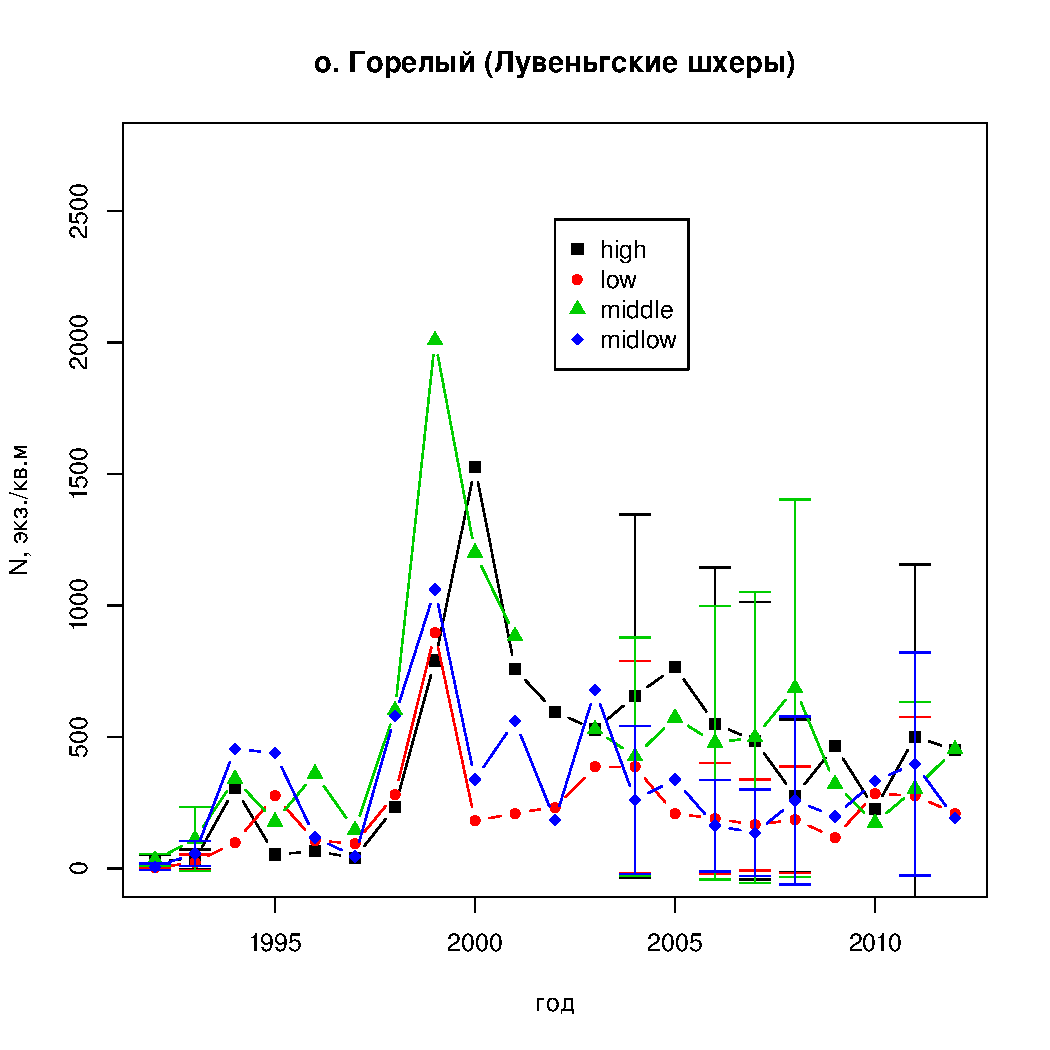
\includegraphics[width=65mm]{../White_Sea/Luvenga_Goreliy/N2_dynamic.pdf}
	\end{center}
	\end{minipage}
%
	\hfil %Это пружинка отодвигающая рисунки друг от друга
%
	\begin{minipage}[b]{.46\linewidth}
%Следующий рисунок - первый ряд справа %DUNGEON S_4 \ AB
	\begin{center}
		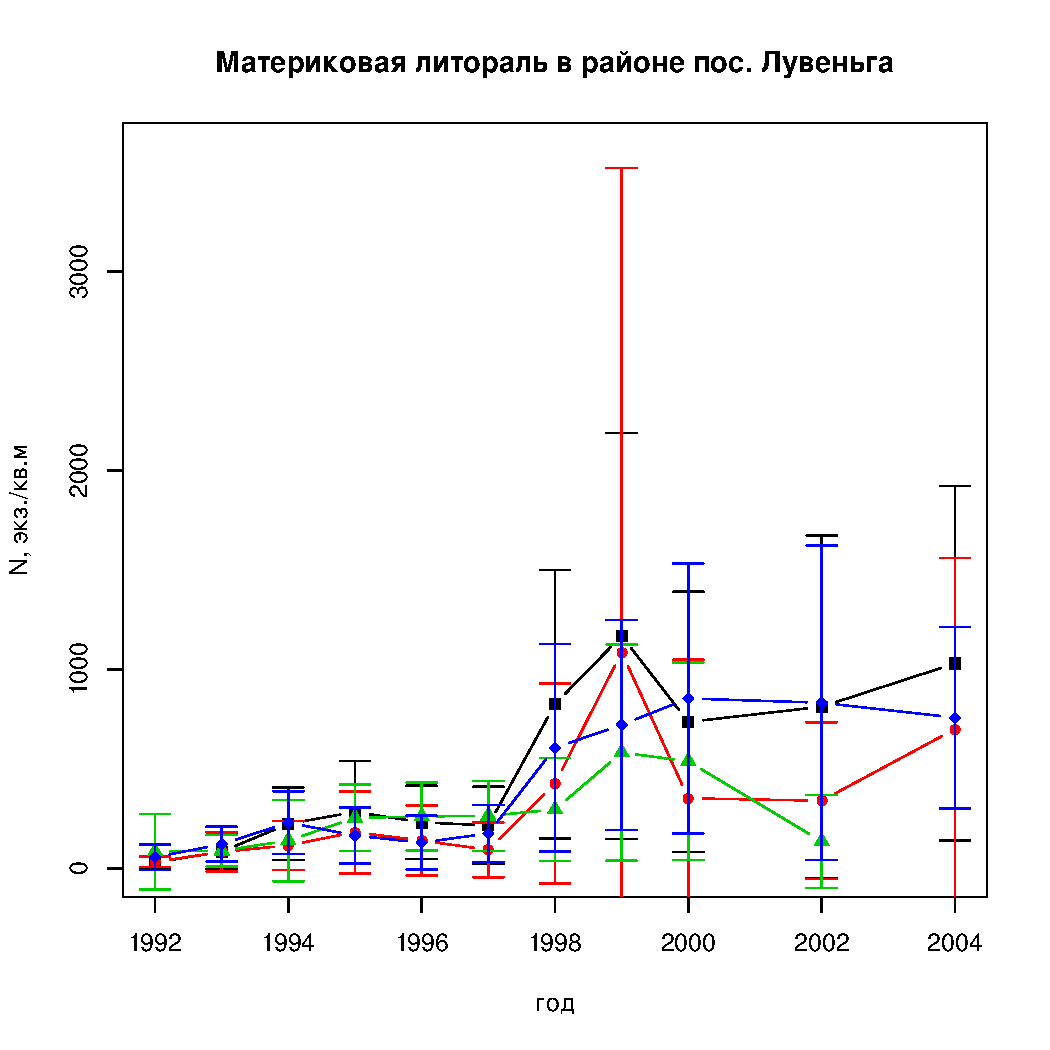
\includegraphics[width=65mm]{../White_Sea//Luvenga_II_razrez/N2_dynamic.pdf}
	\end{center}
	\end{minipage}
	
%\smallskip


	\begin{minipage}[b]{.46\linewidth}
%Фигурка в первом ряду слева размер отведенный под весь этот объект \textendash 0.46 от ширины строки
%Параметр [b] означает, что выравнивание этих министраниц будет по нижнему краю
	\begin{center}
		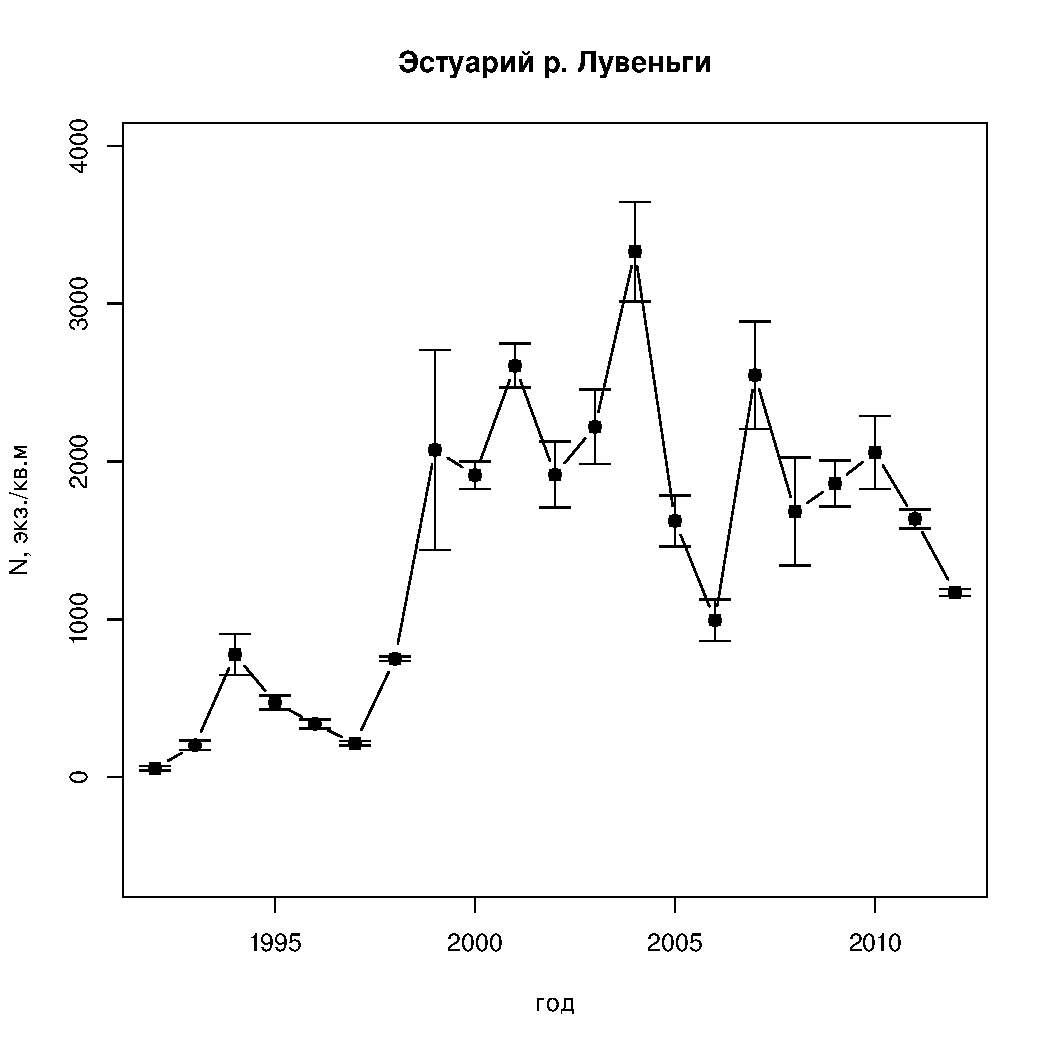
\includegraphics[width=65mm]{../White_Sea/Estuatiy_Luvenga/N2_dynamic.pdf}
	\end{center}
	\end{minipage}
%
	\hfil %Это пружинка отодвигающая рисунки друг от друга
%
	\begin{minipage}[b]{.46\linewidth}
%Следующий рисунок - первый ряд справа %DUNGEON S_4 \ AB
	\begin{center}
		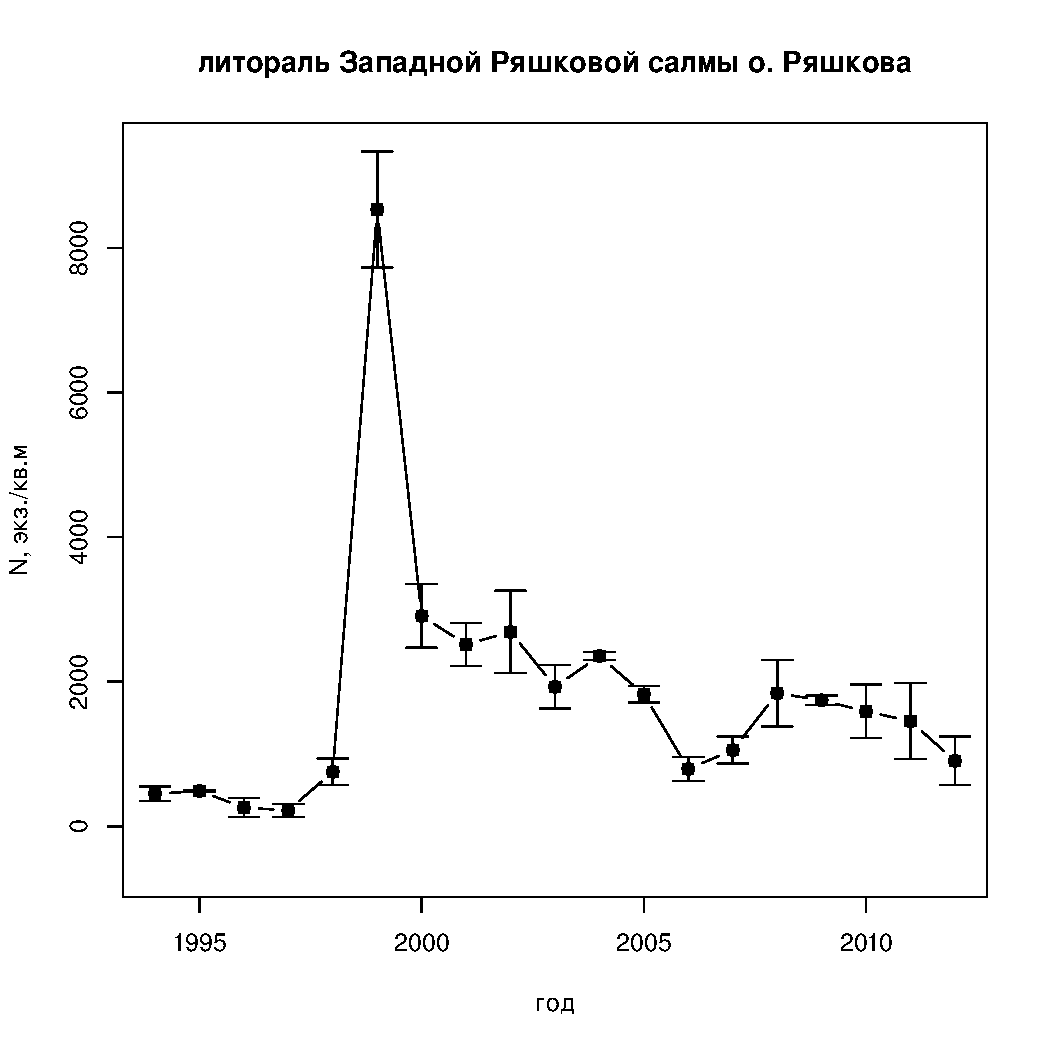
\includegraphics[width=65mm]{../White_Sea/Ryashkov_ZRS/N2_dynamic.pdf}
	\end{center}
	\end{minipage}

%\smallskip

	\begin{minipage}[b]{.46\linewidth}
%Фигурка в первом ряду слева размер отведенный под весь этот объект \textendash 0.46 от ширины строки
%Параметр [b] означает, что выравнивание этих министраниц будет по нижнему краю
	\begin{center}
		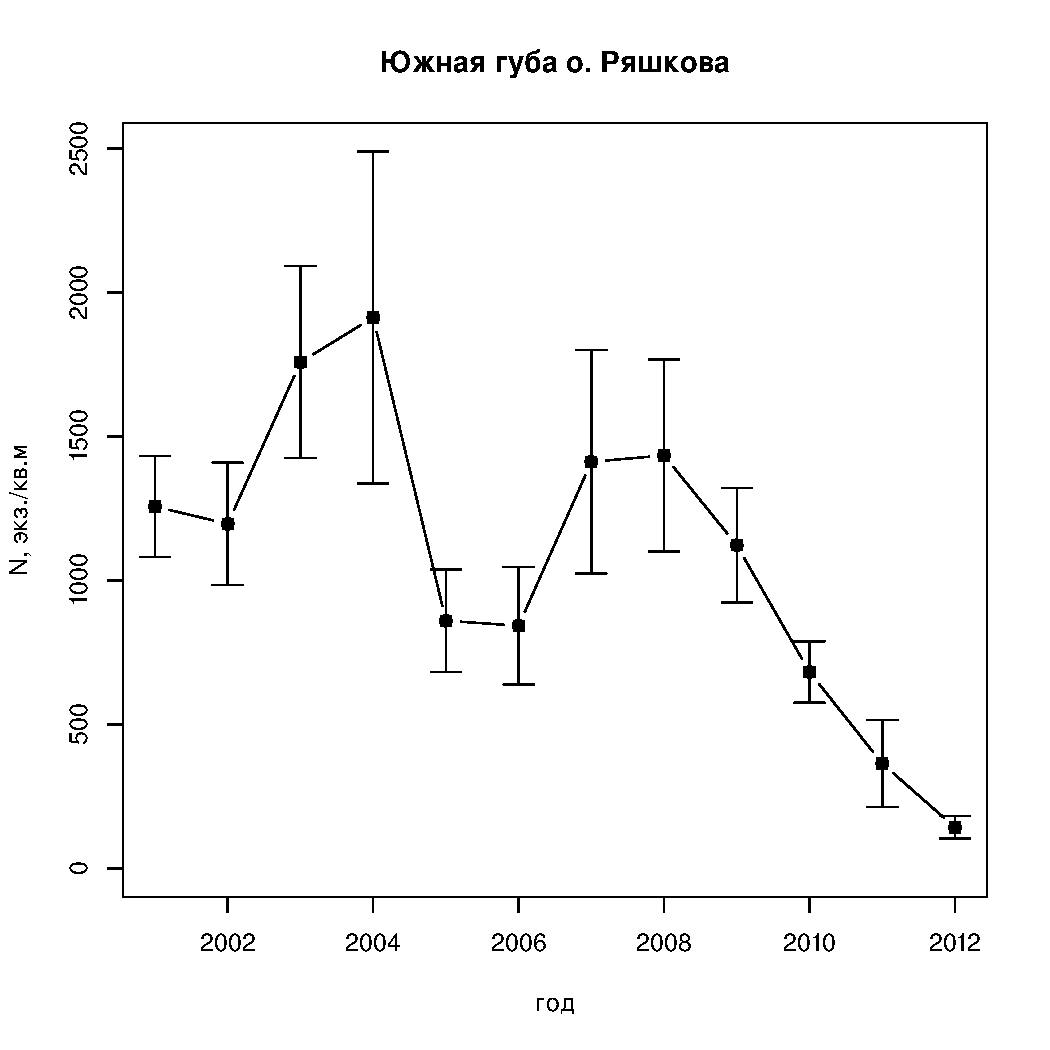
\includegraphics[width=65mm]{../White_Sea/Ryashkov_YuG/N2_dynamic.pdf}
	\end{center}
	\end{minipage}
%
	\hfil %Это пружинка отодвигающая рисунки друг от друга
%
	\begin{minipage}[b]{.46\linewidth}
%Следующий рисунок - первый ряд справа %DUNGEON S_4 \ AB
	\begin{center}
		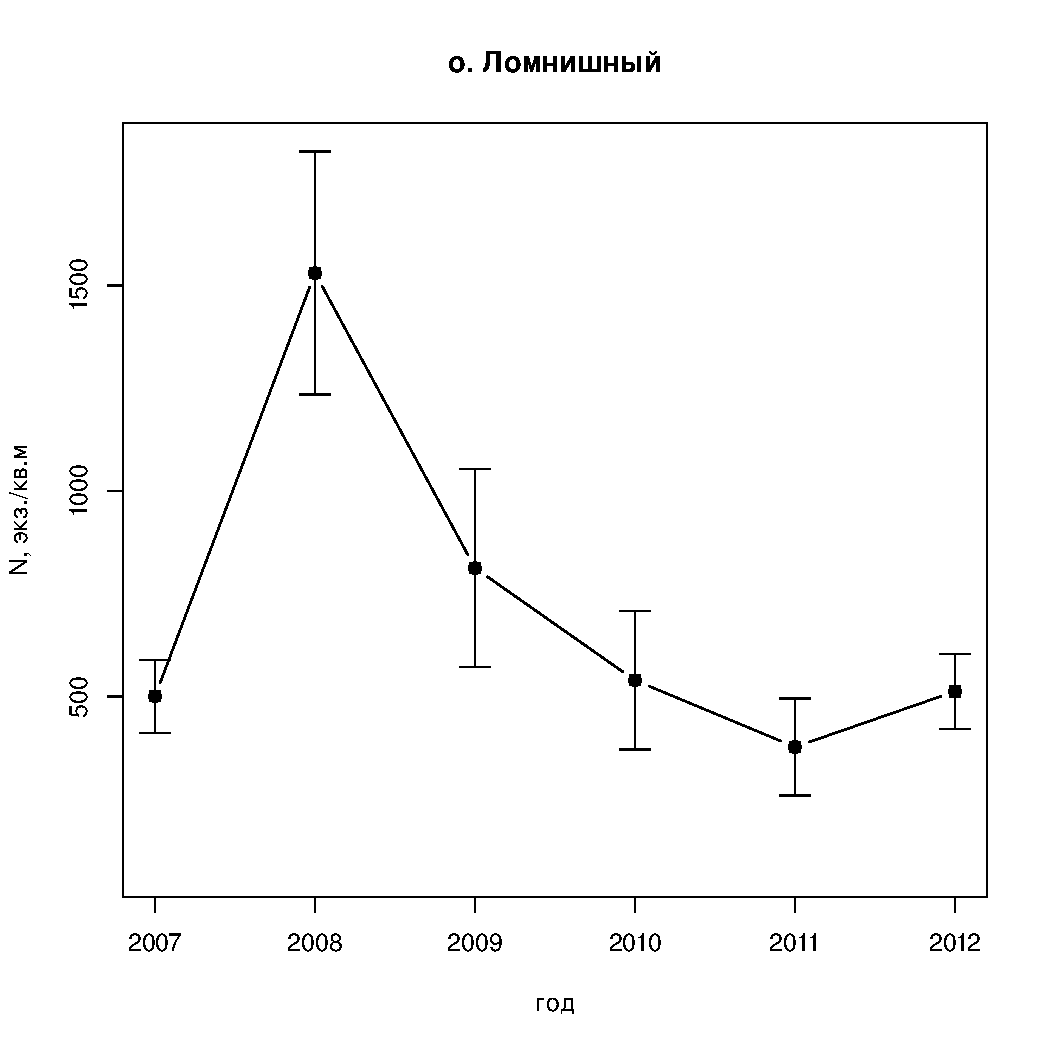
\includegraphics[width=65mm]{../White_Sea/Lomnishniy/N2_dynamic.pdf}
	\end{center}
	\end{minipage}

%\smallskip


	\caption{Динамика численности {\it Macoma balthica} с длиной раковины более $1$~мм в поселениях вершины Кандалакшского залива}
	\label{ris:dynamic_Kandalaksha_all2}
	\end{figure}



Для анализа динамики обилия, на наш взгляд, более информативно рассматривать численность без учета вновь осевших особей. 
\textcolor{red}{ОБЪЯСНЯТЬ ПРО ПОПОЛНЕНИЕ ПОСЕЛЕНИЯ ТУТ ИЛИ ГДЕ?}. 
Поскольку материал собирали в конце июля \textemdash начале августа, то мы считаем спатом всех особей длиной менее $1$~мм. \textcolor{red}{сюда бы ссылку на размер спата в белом? Зубаха, Полоскин, Гольцев? Флячинская?} 
В этом случае можно говорить по крайней мере о двух периодах: с $1992$ по $1998$ год \textemdash период относительно низкой численности (менее $800$~экз./м$^2$ ) моллюсков, и с $1999$ по $2012$ год \textemdash относительно высокой (более $1000$~экз./м$^2$) (достоверные различия по критерию Манна-Уитни, $W = 6, p-value = 4,5 \times 10^{-13}$).

В период с $1992$ по $1998$ год численность {\it M.~balthica} достоверно изменялась ($Kruskal-Wallis\ \chi^2 = 24,1, p-value = 0,00049$). Результаты попарного сравнения представлены в таблице \ref{tab:Tukey_estuary_92_98_n2}.

	\begin{table}
	\begin{tabular}{|*{4}{p{0.2\textwidth}|}} \hline
	годы & различия средних & p-value & достоверность различий\\
	\hline
	$1993-1992$ & $147$ &  $0,11$ & \\
	\hline
	$1994-1993$ & $575$  & $2,47 \times 10^{-7}$ & *** \\
	\hline
	$1995-1994$ & $-303$  & $0,0069$ & ** \\
	\hline
	$1996-1995$ & $-137$  & $0,51$ & \\
	\hline
	$1997-1996$ & $-123$  & $0,62$ & \\
	\hline
	$1998-1997$ & $537$  & $6,73 \times 10^{-6}$ & *** \\
	\hline
	\end{tabular}

	{\footnotesize Примечание: достоверность различий *** \textemdash $p<0,001$; ** \textemdash $p<0,05$; * \textemdash $p<0,1$.}
	\caption{Результаты множественного сравнения средних численностей {\it Macoma balthica} методом Тьюки (Tukey's ‘Honest Significant Difference’) в эстуарии реки Лувеньги в $1992-1998$ годах.}
	\label{tab:Tukey_estuary_92_98_n2}
	\end{table}

Численность моллюсков в эстуарии р. Лувеньги в $1992-1993$ годах оставалась стабильной ($\bar{N} = 128~(21,5)$~экз./м$^2$), затем произошло ее увеличение в $1994$ году, после чего снова произошло некоторое ее снижение и в $1995 - 1997$ годах она стабилизировалась на более высоком уровне ($\bar{N} = 341~(9,3)$~экз./м$^2$) по сравнению с $1992 - 93$ гг.
В $1998$ году вновь происходит увеличение численности {\it M.~balthica} до уровня $1994$ года (около $750 - 800$~экз./м$^2$), после чего в $1999$ году средняя численность возросла ещё в три раза.
С $1999$ по $2003$ год численность оставалась относительно стабильной  ($Kruskal-Wallis\ \chi^2 = 5.0333, p-value = 0.28$) и в среднем составляла $2146~(5,5)$~экз./м$^2$.
В $2004$ году обилие маком увеличилось в полтора раза и достигло максимума для данного участка за весь период наблюдений. 
С $2004$ по $2006$ год численность моллюсков последовательно снижалась (табл.~\ref {tab:Tukey_estuary_04_07_n2}). 
	\begin{table}
	\begin{tabular}{|*{4}{p{0.2\textwidth}|}} \hline
	годы & различия средних & p-value & достоверность различий\\
	\hline
	$2005-2004$ & $-1707$ & $0,09$ & *\\
	\hline
	$2006-2005$ & $-630$ & $0,78$ & \\
	\hline
	$2007-2006$ & $1553$ & $0,05$ & **\\
	\hline
	\end{tabular}

	{\footnotesize Примечание: достоверность различий *** \textemdash $p<0,001$; ** \textemdash $p<0,05$; * \textemdash $p<0,1$.}
	\caption{Результаты множественного сравнения средних численностей {\it Macoma balthica} методом Тьюки (Tukey's ‘Honest Significant Difference’) в эстуарии реки Лувеньги в $2004-2007$ годах.}
	\label{tab:Tukey_estuary_04_07_n2}
	\end{table}
В $2006$ году она достигла локального минимума и составляла $993~(13,2)$~экз./м$^2$). 
В $2007$ году произошло достоверное увеличение численности {\it Macoma balthica} (табл.~\ref {tab:Tukey_estuary_04_07_n2}).
К $2008$ году численность моллюсков снова снижается, после чего до $2012$ года были отмечены недостоверные флуктуации ($Kruskal-Wallis\ \chi^2 = 6,8429, p-value = 0,14$).


		\subsection{Литораль Западной Ряшковой салмы о.~Ряшкова.}

На данном участке литорали средняя плотность поселений {\it M.~balthica} за период с $1994$ по $2012$ год колебалась от $220~(40,9)$~экз./м$^2$ в $1997$ до $9285~(16,4)$~экз./м$^2$ в $1999$~году (рис. \ref{ris:dynamic_Kandalaksha_all}).
При исключение из рассмотрения особей длиной менее $1$~мм минимальная средняя численность не изменилась, а максимальная в $1999$ составила $8530~(9,4)$~экз./м$^2$ (рис. \ref{ris:dynamic_Kandalaksha_all2}).
Однако столь высокая численность не сохранилась дольше одного года, и в период с $2000$ по $2012$ колебалась в пределах $1 \textendash 2,5$~тысяч~экз./м$^2$, в среднем составляя $1823~(8,0)$~экз./м$^2$.
Тем не менее, после $1999$ года средняя численность маком достоверно больше ($W = 4,5, p-value = 1,007 \times 10^{-5}$), чем до \textemdash $2145~(4,5)$ и $435~(17,2)$, соответственно.

Минимальная численность в период после $2000$~года была отмечена в 2006 году и составляла $795~(20,8)$~экз./м$^2$. 
Периоды с $2000$ по $2006$ и с $2007$ по $2012$ годы достоверно различаются ($W = 131,5, p-value = 0,016$) по средней численности маком ($2146~(9,5)$ и $1448~(10,8)$, соответственно).

Внутри каждого периода времени численность {\it M.~balthica} не различается достоверно от года к году (табл. \ref{tab:ZRS_N2_Kruskal}).

	\begin{table}
	\begin{tabular}{|*{4}{p{0.25\textwidth}|}} \hline
	годы наблюдения & $Kruskal-Wallis\ \chi^2$ & $p-value$ & $\bar{N} ~ (D)$ \\ 
	\hline
	$1994 - 1998$ & $7,2$ & $0,12$ & $435~(17,2)$ \\
	\hline
	$2000 - 2006$ & $9,8$ & $0,13$ & $2146~(9,5)$\\
	\hline
	$2007 - 2012$ & $4,9$ & $0,43$ & $1448~(10,8)$ \\
	\hline
	\end{tabular}
	{\footnotesize Примечание: Kruskal-Wallis $\chi^2$ \textemdash значения критерия Краскелл-Уоллиса; $\bar{N}$ \textemdash средняя численность {\it 	M.~balthica}, экз./м$^2$; $D$ \textemdash относительная ошибка средней, \%.}
	\caption{Межгодовое различие численности {\it Macoma~balthica} на литорали Западной Ряшковой салмы о.~Ряшкова в разные годы.}
	\label{tab:ZRS_N2_Kruskal}
	\end{table}


		\subsection{Южная губа острова Ряшкова}
На данном участке с $2001$ по $2010$ год численность {\it Macoma~balthica} была относительно стабильна, все флуктуации были недостоверны ($Kruskal-Wallis chi-squared = 12,07, p-value = 0,21$). 
Средняя численность за данный период составила $1239~(7,9)$~экз./м$^2$.
Однако намечается некоторая тенденция к увеличению численности в $2003-2004$ и $2007-2008$ году.
После $2008$ года численность постепенно снижается и в $2012$ году она составила $142~(27,5)$~экз./м$^2$.

		\subsection{Остров Ломнишный}


\end{document}
